%!TEX root = ../thesis.tex

\section{ネットワークの構造}

  ネットワークを\figref{Fig:okada_network}に示す.これは,深層学習フレームワークであるChainer\cite{chainer}を使用し,CNNをベースとしている.具体的には,入力層,畳み込み層3,全結合層2,出力層の7層で構成されている.深層学習器は,縮小された画像と選択された行動を0.6秒周期で収集して学習する.これに使用されたハイパーパラメータを\tabref{tab:Parameters of network configured with chainer}に示す.

  \begin{figure}[h]
    \centering
    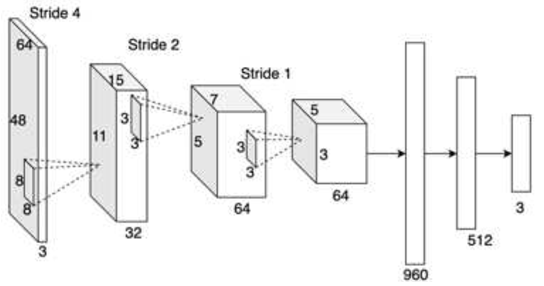
\includegraphics[keepaspectratio, scale=0.70] {images/pdf/okada_network}
    \caption[Structure of the network]{Structure of the network (source: \cite{okada})}
    \label{Fig:okada_network}
  \end{figure}

  \begin{table}[hbtp]
    \caption{Parameters of network configured with chainer}
    \label{tab:Parameters of network configured with chainer}
    \centering
    \begin{tabular}{cc}
      \hline
      Input data & Image(64x48 pixels, RGB channels) \\
      Optimizer & Adam($alpha = 0.001, beta1 = 0.9, beta2 =  0.999, pdf = 1e^{-2}$)\\
      Loss function & Softmax-cross-entropy\\
      Output data & Action (Forward, Turn Left, Turn Right)\\
      \hline
    \end{tabular}
  \end{table}

\newpage